%
%
\chapter{Moderna}

\begin{enumerate}[start=1,label={\bfseries Q\arabic*.}]

\item Uma batalha espacial entre duas naves de civilizações diferentes, A e B, em repouso uma em relação à outra, acaba em destruição mútua. Um observador C, em repouso em relação às duas naves e para quem a distância entre elas era $L$, observa a nave da civilização A explodir um tempo $T$ antes da explosão da outra nave. Um outro observador D move-se com velocidade de magnitude $u$ em relação ao primeiro observador, ao longo da linha que separava as duas naves.


a) Supondo uma situação em que $L = 1.000 km$ e $u = \frac{24}{25}c$, sendo $c$ a velocidade da luz no vácuo, qual era a distância entre as naves no referencial do observador $D$?

    {\color{red}
    O observador $D$ observa um comprimento $L'$ relacionado a $L$ através da contração de Lorentz,

    $$
    L' = L \sqrt{1 - \frac{u^{2}}{c^{2}}}.
    $$

    Substituindo os valores do enunciado, $L' = 280 \ km$.


    }

b) Em outra situação, supondo $L = 1.000 km$ e $T = 1 ms$, qual deveria ser a magnitude mínima da velocidade $u$ para que o observador D registrasse a explos˜ao da nave da civilização B como tendo ocorrido antes da explosão da nave da civilização A?

    {\color{red}

    Supondo, sem perda de generalidade, que as naves situam-se ao longo do eixo $x/x'$ em ambos os referenciais de C e D, e que as origens destes coincidem no instante $t = t' = 0$, os referenciais relacionam-se pela transformação de Lorentz

    $$
    x^{\prime} = \gamma (x - ut) \quad \ \ \ t^{\prime} = \gamma \left( t - \frac{u}{c^{2}} x \right),
    $$

    com

    $$
    \gamma = \frac{1}{\sqrt{1-\frac{u^{2}}{c^{2}}}}
    $$

    Denotando por 1 e 2 as explosões das naves das civilizações A e B, respectivamente, temos


    \begin{eqnarray*}
    % \nonumber % Remove numbering (before each equation)
      \Delta x &=& x_{2} - x_{1} = L \quad \ \ \ \quad \Delta t = t_{2} - t_{1} = T, \\
      \Delta t' &=& t'_{2} - t'_{1} = \gamma \left(  \Delta t - \frac{u}{c^{2}} L \right).
    \end{eqnarray*}

    Para que o observador D registre o evento 2 como anterior ao evento 1, é preciso que

     $$
     \Delta t' < 0 \Rightarrow T - \frac{u}{c^{2}} L < 0,
     $$

    ou seja,

    $$
    u > \frac{c^{2}T}{L} = 9 \times 10^{4} km/s.
    $$

    }


c) Considere que toda a energia de repouso da nave da civilização A tenha sido liberada na explos˜ao e que o veículo do observador C tenha capturado toda essa energia, convertendo-a em energia cinética. Sendo iguais as massas da nave da civilização A e a do veículo de C, determine a velocidade $v$ que o veículo atinge após absorver a energia da explos˜ao.

{\color{red}

$$
m_{A} c^{2} = \frac{m_{C} c^{2}}{\sqrt{1-\frac{v^{2}}{c^{2}}}} - m_{C} c^{2}.
$$

Portanto,


$$
\begin{aligned}
& \sqrt{1-\frac{v^{2}}{c^{2}}}=\frac{m_{C}}{m_{A}+m_{C}} \Rightarrow \frac{v^{2}}{c^{2}} = 1-\left(\frac{m_{C}}{m_{A}+m_{C}}\right)^{2}\\
& v = c \sqrt{1 - \left(\frac{m_{C}}{m_{A}+m_{C}} \right)^{2}}
\end{aligned}
$$

com $m_{A} = m_{C}$, obtemos

$$
v = \sqrt{\frac{3}{4}}c.
$$

}








\item A superfície do Sol está a uma temperatura aproximada de $6,0 \times 10^{3} \ K$, enquanto a superfície da estrela supergigante Betelgeuse está a uma temperatura aproximada de $3,0 \times 10^{3} \ K$. Suponha que ambas as estrelas irradiem como corpos negros perfeitos.


  a) A radiância espectral é definida como a energia irradiada por unidade de tempo e por unidade de área da superfície de um corpo no intervalo de comprimentos de onda entre $\lambda$ e $\lambda + d\lambda$. Qual é a razão entre o comprimento de onda para o qual a radiância espectral do Sol é máxima e o comprimento de onda correspondente para Betelgeuse?

  {\color{red}

  Pela lei do deslocamento de Wien, o produto da temperatura de um corpo negro pelo comprimento de onda que maximiza sua radiância espectral é constante. Logo, para o Sol (S) e Betelgeuse (B) vale

$$
\lambda_{S} T_{S} = \lambda_{B} T_{B} \Rightarrow = \frac{\lambda_{S}}{\lambda_{B}} = \frac{T_{B}}{T_{S}} = \frac{3,0 \times 10^{3}}{3,0 \times 10^{3}} = \frac{1}{2}.
$$


  }


  b) Qual é a razão entre a radiância (energia total irradiada por unidade de tempo e de área da superfície) na superfície do Sol e a radiância na superfície de Betelgeuse?

  {\color{red}

Pela lei de Stefan-Boltzmann, a radiância a partir da superfície de um corpo negro é proporcional à quarta potência de sua temperatura absoluta, com uma constante de proporcionalidade universal. Logo, para o Sol e Betelgeuse vale

$$
\frac{I_{B}}{T_{B}^{4}} = \frac{I_{S}}{T_{S}^{4}} \Rightarrow \left( \frac{T_{S}}{T_{B}}  \right)^{4} = \left( \frac{6,0 \times 10^{3}}{6,0 \times 10^{3}} \right)^{4} = 16.
$$

}


  c) A potência de radiação de Betelgeuse é de cerca de $4,0 \times 10^{4}$ vezes a potência de radiação do Sol. Estime a razão entre o raio de Betelgeuse e o raio do Sol.

  {\color{red}

Ainda pela lei de Stefan-Boltzmann, e da definição de radiância como potência ($P$) por unidade de área ($A$), temos

$$
\frac{I_{B}}{I_{S}} = \frac{P_{B}/A_{B}}{P_{S}/A_{S}} = \left( \frac{T_{B}}{T_{s}}  \right)^{4}.
$$

Levando em conta que a área superficial de uma estrela é proporcional ao quadrado de seu raio,

$$
\frac{P_{B}/R_{B}^{2}}{P_{S}/R_{S}^{2}} = \frac{P_{B}}{P_{S}} \left( \frac{R_{S}}{R_{B}} \right)^{2} = \left( \frac{T_{B}}{T_{s}}  \right)^{4},
$$


donde

$$
\frac{R_{B}}{R_{S}} = \sqrt{\frac{P_{B}}{P_{S}}} \left( \frac{T_{S}}{T_{B}} \right)^{2} = \sqrt{4 \times 10^{4}} \left( \frac{6,0 \times 10^{3}}{6,0 \times 10^{3}}  \right)^{2} = 8,0 \times 10^{2}.
$$

}



\item O gráfico da fígura abaixo representa a emitância espectral, $e(\lambda)$, de um corpo negro a uma tempretura $T_{1}$ como funão do comprimento de onda $\lambda$. A energia radiada por unidade de tempo e por unidade de área do corpo, na faixa de comprimentos de onda entre $\lambda$ e $\lambda + d \lambda$, é dada por $e(\lambda)d\lambda$. No gráfico, $\lambda$ é dado em nanometros ($1 \ nm = 10^{-9} \ m$) e a emitância espectral é dada em unidades arbitrarias.



  a) Com base no gráfico, estime a temperatura $T_{1}$.

  \resposta

  b) Calcule a energia total radiada por unidade de tempo e por unidade de área desse corpo negro. Expresse o resultado em $W/m^{2}$.

  \resposta

  c) A partir do gráfico, calcule, calcule aproximadamente a energia radiada por unidade de tempo e por unidade de área do corpo, na faixa de comprimentos de onda entre 6000 $nm$ e 8000 $nm$. Expresse o resultado em $W/m^{2}$.

  \resposta

  d) Considere agora um segundo corpo negro a uma temperatura $T_{2} = 3T_{1}$. Determine o comprimento de onda de máxima emitância espectral desse segundo corpo (em $nm$).




\item O acelerador de partículas LHC ("Large Hadron Collider") produz feixes de protóns com velocidades relativistiscas e energias (medidas no referencial do laboratório, $ S $) da ordem de teraelétron-volts ($ 1,0 TeV = 1,0 \times 10^{12} eV $).


  a) Um próton possui energia relativística total igual a $5,0 \ TeV$, medida no referencial $ S $ do laboratório. Calcule a velocidade desse próton (no referencial $ S $) considerando-se que a sua energia de repouso é igual $1,0 \ GeV = 1,0 \times 10^{9} \ eV $. \textit{Dica}: como a velocidade do próton é muito próxima à velocidade da luz no vácuo, c, use $v = (1 - \Delta)c$ e encontre o valor de $\Delta$. Lembre-se que $\sqrt{1-\mathcal{E}} \simeq 1 - \frac{\mathcal{E}}{2}$ se $\mathcal{E} << 1$.

  \resposta

  b) Um próton $A$, com energia relativística total $E_{A}$, colide frontamente com outro próton $B$ com a mesma energia e viajando em sentido contrário no referencial $ S $. Suponha que esta colisão produza uma partícula $X$ não vista anteriormente através da reação $A+B \Rightarrow X$. Calcule a massa de repouso da partícula $X$ em termos de $E_{A}$.

  \resposta

  c) Em outro experimento, um próton $C$, com fator relativístico $\gamma$ (medido no referecial do laboratório $S$) e massa de repouso $m_{0}$, colide frontalmente com outro próton $D$ inicalmente em repouso. Suponha que esta colisão produza uma partícula $Y$ através da reação $C+D \Rightarrow Y$. Calcule a massa de repouso de $Y$ em termos de $\gamma$ e $m_{0}$.

  \resposta



\item Raios cósmicos que atingem a atmosfera terrestre dão origem a uma cascata de partículas com diversas energias, entre elas os múons. Múons são instáveis e decaem espontaneamente segundo a lei $N(t) = N_{0} e^{-t/\tau}$, onde $N(t)$ e $N_{0}$ são os números instáveis e decaem nos instantes $t$ e $t=0$, respectivamente, e $\tau$ é o tempo de vida do múon, cujo valor é $\tau = 2,0\mu s$, quando medido no seu referencial próprio. Um detector $D_{1}$ de múons seletivo em velocidade é montado no topo de uma montanha a $2,94 \times 10^{3}\ m$ acima do nível do mar. O detector é ajustado para detectar partículas com velocidade $v = 0,98c$. Num certo intervalo de tempo, são detectados $1,5 \times 10^{3}$ múons. Em um outro detector semelhante $D_{2}$, montado ao nível do mar, faz-se a mesma medida (mesma velocidade e mesmo intervalo de tempo) e obtém-se um número de múons que é ordens de grandeza maior que o valor esperado segundo a física não relativística.


  a) Determine o número de múons que seria esperado no detector $D_{2}$, segundo a física não relativística.

\resposta Segundo a física não relativística, o tempo gasto pelos múons para percorrer os 2940 $m$ do topo da montanha até o nível do mar (distância medida no referencial de $D_{2}$) é
$$
t = \frac{2,94 \times 10^{3}}{0,98 \times 3,0 \times 10^{8}} = 1,0 \times 10^{-5} s = 10 \mu s.
$$
Desta forma, segundo o cálculo não relativístico, o número de múons detectados ao nível do mar seria
$$
N_{n-rel}(t = 10 \mu s) = 1,5 \times 10^{3} e^{(-10/2,0)} \approx 10.
$$


  b) Explique \textit{qualitativamente} por que o número observado no detector $D_{2}$ é maior que a expectativa não relativística.

\resposta O enunciado informa que a contagem medida é ordens de grandeza maior do que o esperado segundo a física não relativística. A razão da discrepância é o fato de que os múons detectados são partículas relativísticas ($v \approx c$) e efeitos relativísticos devem ser levados em conta, como a
dilatação temporal e/ou a contração dos comprimentos.

  c) Calcule a contagem de múons no detector $D_{2}$: (i) do ponto do vista de um observador no referencial preso ao detector e (ii) do ponto de vista de um observador no referencial próprio dos múons.

\resposta  (i) Tratando agora o sistema relativisticamente, o tempo de vida dos múons, no sistema de referência de $D_{2}$, não é $\tau = 2,0 \mu s$, mas sim $\tau_{D_{2}} = \gamma \tau$, com $\gamma = 1 / \sqrt{1 - v^{2}/c^{2} }$, devido ao efeito de dilatação do tempo. Para o grupo de múons relevantes para o experimento, $\gamma \approx 5,0$ e $\tau_{D_{2}} \approx 10 \mu s$. Portanto,
$$
N(t = 10 \mu s) = 1,5 \times 10^{3} e^{(-10/10)} \approx 5,5 \times 10^{2}.
$$
contagem que, de fato, é 2 ordens de grandeza maior do que aquela prevista pela física não relativística.

(ii) Do ponto de vista de um observador que viaja junto com os múons, o que ocorre é que ele não mede uma distância percorrida de $d = 2,94 \times 10^{3} \ m$, mas sim uma distância $d' = d/\gamma \approx 5,9 \times 10^{2} \ m$, pela contração dos comprimentos. Desta forma, o tempo gasto pelos múons para
percorrer esta distância será
$$
t' = \frac{d'}{v} = \frac{5,9 \times 10^{2}}{0,98 \times 3,0 \times 10^{8}} = 2,0 \mu s.
$$
Logo,
$$
N'(t = 2,0 \mu s) = 1,5 \times 10^{3} e^{(-2,0/2,0)} \approx 5,5 \times 10^{2}.
$$
Um observador viajando com os múons medirá uma contagem dos mesmos $5,5 \times 10^{2}$ múons medidos por um observador do grupo de físicos, no nível do mar.


  d) Considere um referencial inercial $S$, no qual tanto os múons quanto o detector $D_{2}$ estão em movimento, aproximando-se com velocidade de módulos iguais. Do ponto de vista de um observador no referencial $S$, o número de múons observado no detector $D_{2}$ é menor, maior ou igual ao do item (c)? Justifique sua resposta.

\resposta A resposta será igual. Isto é de se esperar, porque números de objetos são invariantes relativísticos.






\item Um feixe de nêutrons formando uma onda de materia de comprimento de onda $\lambda$ incide sobre um cristal fazendo um ângulo $\theta \in [0, \pi/2]$ com os planos cristalinos. A distância entre dois planos cristalinos adjacentes é $d$, como mostrado na figura. A energia de repouso do nêutron é $E_{n}^{0} = 940 MeV$.
\begin{figure}[H]
  \centering
  \includegraphics[scale=0.7]{moderna-img/espalha}
\end{figure}


  a) Deduza a expressão que relaciona $\lambda$, $\theta$ e $d$ e que descreve a reflexão de Bragg.

  \resposta
\begin{figure}[H]
  \centering
  \includegraphics[scale=0.7]{moderna-img/espalha1}
\end{figure}
Da geometria do diagrama acima, a diferença de caminho óptico entre os raios refletidos nos planos superior e inferior é $2d \sin \theta$. A condição de interferência construtiva entre os raios é obtida impondo que a diferença de caminho óptico seja um múltiplo inteiro $n$ do comprimento de onda: $n\lambda = 2d \sin \theta$.


b) Um cristal tem planos cristalinos separados por $d = 1,1 \ \AA $. Usando nêutrons com energia cinética $K = 1,9 eV$, em quantos valores diferentes de $\theta$ é observada a reflexão de Bragg?

\resposta  O comprimento de onda da onda de matéria associada aos nêutrons é
$$
 \lambda=\frac{h}{m v}=\frac{h}{\sqrt{2 m K}}=\frac{h c}{\sqrt{2 K m c^{2}}}=\frac{1.240 \mathrm{eV} . \mathrm{nm}}{\sqrt{2 \times 1,9 \times 9,4 \times 10^{8} \mathrm{eV}^{2}}}=0,21 \AA
$$
O maior ângulo de reflexão de Bragg que pode ocorrer é de $\theta = \pi/2$, para o qual $2d \sin(p/2)$ e $n = 2d/\lambda$. Usando o valor de $d$ fornecido obtemos $n = 10,5$. Como $n$ deve ser um inteiro, a mais alta ordem observada é a décima ($n = 10$).



c) Explique como um cristal pode ser usado como filtro para selecionar velocidades de nêutrons a partir de um feixe com uma distribuição larga de velocidades.

\resposta A dispersão de velocidades dos nêutrons se traduz em uma dispersão de comprimentos de onda de de Broglie presentes no feixe de partículas. Assim, para um determinado ângulo de incidência do feixe de partículas, haverá um intervalo de ângulos de reflexão $\varphi$ para cada ordem $n$ de reflexão. Fixando-se um filtro espacial (uma fenda, por exemplo) em torno de um ângulo de detecção bem definido $\varphi_{det}$, estaremos deixando passar pelo aparato apenas os nêutrons cuja velocidade esteja relacionada com o comprimento de onda de de Broglie que satisfaz à condição $n\lambda = 2d \sin \varphi_{det}$, selecionando assim uma certa velocidade.


d) As relações $E = h\nu$ e $p = h/\lambda$ também são válidas no regime relativístico, sendo $E$ a energia relativística total da partícula, $p$ o seu momento linear e $\lambda$ e $\nu$ o comprimento de onda e a frequência da onda de matéria associada, respectivamente. Encontre a \textbf{velocidade de fase} de uma onda de matéria associada a nêutrons relativísticos em termos de $E_{n}^{0}$ e $\lambda$. O resultado é maior, menor ou igual à velocidade da luz no vácuo? Encontre também a \textbf{velocidade de grupo} da onda, compare com a velocidade de fase e comente os resultados.

\resposta A velocidade de fase pode ser escrita como
$$
v_{f}=\lambda \nu=\frac{\lambda E}{h}=\frac{\lambda}{h} \sqrt{p^{2} c^{2}+\left(E_{n}^{0}\right)^{2}}=\frac{\lambda}{h} \sqrt{\frac{h^{2} c^{2}}{\lambda^{2}}+\left(E_{n}^{0}\right)^{2}}=c \sqrt{1+\left(\frac{\lambda E_{n}^{0}}{h c}\right)^{2}}>c
$$
onde usamos $E^{2} = p^{2}c^{2} + m^{2}c^{4} = p^{2}c^{2} + (E_{0}^{n})^{2}$. Por outro lado, a velocidade de grupo é dada por
$$
v_{g}=\frac{d \omega}{d k}=\frac{d \nu}{d\left(\lambda^{-1}\right)}=\frac{1}{h} \frac{d E}{d\left(\lambda^{-1}\right)}=\frac{1}{h} \frac{d}{d\left(\lambda^{-1}\right)} \sqrt{\frac{h^{2} c^{2}}{\lambda^{2}}+\left(E_{n}^{0}\right)^{2}}
$$
onde a última expressão para a energia total relativística foi obtida no cálculo de $v_{f}$. Tomando a derivada
$$
v_{g}=\frac{1}{h} \frac{h^{2} c^{2}}{\lambda} \frac{1}{\sqrt{\frac{h^{2} c^{2}}{\lambda^{2}}+\left(E_{n}^{0}\right)^{2}}}=\frac{c}{\sqrt{1+\left(\frac{\lambda E_{n}^{0}}{h c}\right)^{2}}}<c
$$
Conclui-se que $v_{f}v_{g} = c^{2}$. Uma partícula pode ser descrita na física quântica associando-a a um pacote de ondas formado pela superposição infinita de ondas planas, cada qual se movendo com uma velocidade $v_{f}$ , que pode ser maior do que $c$. O pacote de ondas se move com velocidade $v_{g}$. Como é o pacote de ondas (e não as ondas planas que o formam) que carrega informação, sua velocidade não pode exceder a velocidade da luz, como de fato encontramos.




\item A figura \textbf{a} abaixo [ retirada do artigo Wave-particle duality of $C_{60}$ molecule de M. Arndt et al., Nature \textbf{401}, 680 (1999) ] mostra o padrão de difração obtido pela passagem de um feixe de moléculas de fulereno ($C_{60}$) por uma grade de difração. Ela mostra a contagem de moléculas no detector versus a posição vertical $y$ (em $\mu m$) medida a partir da interseção da direção do feixe com o plano do detector, como mostrado esquematicamente na figura \textbf{b}. O plano do detector estava a uma distância de $1,25 \ m$ da grade de difração.

\begin{figure}[H]
  \centering
  \includegraphics[scale=0.5]{moderna-img/carbono.png}
  \includegraphics[scale=0.5]{moderna-img/carbonoespa.png}
\end{figure}


  a) A partir dos dados do gráfico, estime a posição $y_{1}$ do primeiro pico ao lado do máximo central de difração e determine o ângulo $\theta_{1}$ correspondente.

  \resposta

  b) Ao ver o padrão de difração, uma estudante supôs que se tratava de uma padrão de interferência de uma onda eletromagnética passando por uma fenda dupla. Ela foi informada de que o espaço entre as fendas era de $100\ nm$. A partir dessas hipóteses e com base no ângulo do primeiro pico obtido no item (a), calcule o comprimento de onda $\lambda$ da onda incidente.

  \resposta

  c) Sabendo que a velocidade de cada molécula de $\mbox{C}_{60}$ no feixe é de $220\ m/s$, calcule o módulo do momento linear da molécula. A massa molar do carbono é $12 \ g/mol$.

  \resposta

  d) Utilizando o resultado do item (c), calcule o comprimento de onda de de Broglie de uma molécula de $\mbox{C}_{60}$ no feixe.

  \resposta




\item A figura abaixo mostra a intensidade dos raios-X espalhados $I(\lambda)$ com comprimento de onda $\lambda$ por um alvo de grafite no famoso experimento de Compton de 1923. Os raios-X são detectados a um ângulo $\theta$ fixo em relação à direção de incidência no alvo. Parte dos fótons sofre espalhamento elástico (sem perda de energia) e outra parte sofre espalhamento Compton. Como resultado, nota-se que $I(\lambda)$ apresenta dois pics em comprimentos de onda $\lambda_{1}$ e $\lambda_{2} > \lambda_{1}$.

\begin{figure}[H]
  \centering
  \includegraphics[scale=0.7]{moderna-img/raiosx}
\end{figure}


  a) Qual o comprimento de onda dos raios X incidentes e o dos raios X que sofreram espalhamento Compton? Justifique sua resposta.

  \resposta

  Considere um evento de espalhamento Compton em que a energia do fóton incidente no alvo é de $23 \ keV$ e o ângulo de espalhamento é $\theta = 60º$.

  b) Calcule o comprimento de onda do fóton incidente.

  \resposta

  c) Calcule o comprimento de onda do fóton espalhado.

  \resposta

  d) Calcule a energia cinética do elétron após o espalhamento.

  \resposta




\item Um \textbf{positrônio} é um estado ligado entre um elétron (carga $-e$ e massa $m_{e}$) e um anti-elétron (pósitron). A aplicação do modelo de Bohr para este sistema supõe órbitas clássicas circulares do elétron e do pósitron.


a) Supondo órbitas circulares e trabalhando no referencial do centro de massa, calcule a expressão clássica do momento angular $L$ do sistema em função de $e$, $m_{e}$, $\epsilon$ e a distância $R$ entre o elétron e o pósitron.

\resposta

b) Aplique a regra de quantização de Bohr ao positrônio e deduza a expressão para os valores $R_{n}(n = 1 2,3,...)$ dos raios permitidos das órbitas, em termos do raio de Bohr.

\resposta

c) Calcule as energias permitidas pela regra de Bohr $E_{n}$ $(n = 1,2,3,...)$ em elétron-volts.

\resposta

d) Considere agora uma transição do primeiro estado excitado ($n = 2$) para o estado fundamental ($n = 1$) do positrônio (inicialmente em repouso no referencial do laboratório), seguida da emissão de um fóton. Calcule a velocidade do centro de massa $v_{cm}$ do positrônio no referencial do laboratório após a transição. Considere que $v_{cm} << c$ e despreze a energia cinética de recuo do positrônio em relação à energia do fóton.

\resposta






\item O processo de \textbf{espalhamento Compton inverso} é um dos mecanismos para a produção de fótons de alta energia a partir da colisão entre elétrons relativísticos e fótons de baixa energia. Um exemplo é o caso de elétrons de altas energias que se propagam pelo espaço e podem colidir com fótons da radiação cósmica de fundo, gerando fótons na região de raios-X.



a) Supondo que a radiação cósmica de fundo apresenta a distribuição espectral de um corpo negro a uma temperatura $T = 2,9 \ K$, estime o comprimento de onda correspondente ao máximo da distribuição.

\resposta

b) Calcule a frequência (em $Hz$) e a energia (em $eV$) de um fóton cujo comprimento de onda corresponde ao calculado no item (a).

\begin{figure}[H]
  \centering
  \includegraphics[scale=0.8]{moderna-img/positron.png}
\end{figure}

\resposta

Considere o processo de espalhamento Compton inverso entre um elétron e um fóton esquematizado na figura acima. A energia do fóton incidente é $E_{i}$. Após a colisão, o elétron (ainda em movimento) tem energia final menor do que a inicial enquanto o fóton resultante é mais energético ($E_{f} > E_{i}$).

c) Calcule a energia $E_{f}$ do fóton após o espalhamento em termos de $E_{i}$, do fator $\gamma$ relativístico do elétron incidente e da energia de repouso do elétron $m_{e}c^{2}$

\resposta

d) Considere que o fóton incidente faz parte da radiação cósmica de fundo [com energia calculada no item (b)] e o elétron tenha inicialmente uma energia de 250 $MeV$. Calcule a energia do fóton espalhado em $eV$ com dois algarismos significativos. Você pode utilizar $(1 — x^{2})^{\frac{1}{2}} \approx 1 - \frac{x^{2}}{2}$ para x << 1.

\resposta




\item A densidade de energia $u(T)$ da radiação eletromagnética em equilíbrio térmico à temperatura $T$ pode ser expressa (a partir de argumentos termodinâmicos) como

\begin{equation}
u(T) = \int_{0}^{\infty} \nu^{3} f \left( \frac{\nu}{T} \right) d \nu
\end{equation}


onde $\nu$ é a frequência da radiação.




a) \textbf{Apenas usando a Eq.} (1), encontre $u(T)$ a menos de um fator (independente de $T$). Qual é a dimensão deste fator?

\resposta  Fazendo a mudança de variáveis $\nu=x T$, na expressão para a densidade de energia, fornecida no enunciado, obtém-se
$$
u(T)=T^{4} \int_{0}^{\infty} x^{3} f(x) d x . \equiv K T^{4}
$$
onde $K$ é uma constante independente da temperatura. Como $u$ tem dimensão de energia por unidade de volume, segue que $K$ tem dimensão de energia por unidade por unidade de temperatura absoluta à quarta potência ou
$$
[K]=\frac{[E]}{l^{3} k^{4}}=\frac{m}{l t^{2} k^{4}}
$$
onde $m$ tem dimensão de massa, $l$ tem dimensão de comprimento, $t$ tem dimensão de tempo e
$k$ tem dimensão de temperatura absoluta e usamos que $[E]=m l^{2} / t^{2}$


b) Em 1900, Planck descobriu que
$$
u(T) = \int_{0}^{\infty} \nu^{3} f \left( \frac{\nu}{T} \right) = \frac{8 \pi \nu^{2}}{c^{3}} \frac{h\nu}{e^{h\nu / k_{B}T} - 1},
$$
onde $h$ é a constante de Planck (que relaciona o quantum de energia e a frequência, $c$ é a velocidade da luz no vácuo e $k_{B}$ é a constante de Boltzmann.



\item[(i)] Discuta, sem demonstrar, o significado físico do fator $\frac{8\pi \nu^{2}}{c^{3}} d \nu$.

\resposta O fator $\frac{8 \pi \nu^{2}}{\text { for }} d \nu$ é número de modos normais de vibração do campo eletromagnético, por unidade de volume, com frequência no intervalo $[\nu, \nu+d \nu]$


\item[(ii)] Determine o comportamento da distribuição de energia no limite em que a energia do fóton é muito menor do que a energia térmica $k_{B}T$.

\resposta Se $h \nu \ll k_{B} T, \exp \left(h \nu / k_{B} T\right) \approx 1+h \nu / k_{B} T$ e a distribuição de energia é
$$
\frac{h \nu}{\mathrm{e}^{\left(h \nu / k_{B} T\right)}-1} \approx \frac{h \nu}{\frac{h \nu}{k n T}}=k_{B} T
$$


\item[(iii)] Qual é o significado do resultado do item (ii) no contexto da física clássica?

\resposta O resultado obtido no item anterior é o que seria obtido utilizando um tratamento clássico,
via o teorema de equipartição para osciladores clássicos: $k_{B} T / 2$ para cada termo quadrático na energia, termo cinético e potencial harmônico.




c) As constantes $c$, $\hbar = h/(2\pi)$ e a constante gravitacional $G$ podem ser usadas para definir unidades absolutas de tempo ($t_{P}$), distância ($l_{P}$) e massa ($m_{P}$). Determine essas grandezas em termos de produtos de potências de $\hbar$, $c$ e $G$. Determine também a temperatura de Planck $T_{P}$. Estime a ordem de grandeza de $t_{P}$ , $l_{P}$ , $m_{P}$ e $T_{P}$ no sistema internacional de unidades.
\resposta Determinamos primeiramente $t_{P} .$ Escrevendo, de maneira geral,
$$
t_{P}=G^{\alpha} h^{\beta} c^{\gamma}
$$
e levando em conta que
$$
[G]=l^{3} t^{-2} m^{-1} ;[h]=m l^{2} t^{-1} ; \quad[c]=l t^{-1}
$$
obtém-se $l^{3 \alpha+2 \beta+\gamma} m^{-\alpha+\beta} t^{-2 \alpha-\beta-\gamma}=t$
Logo, $\alpha=\beta=1 / 2$ e $\gamma=-5 / 2 .$ Portanto,
$$
t_{P}=\sqrt{\frac{h G}{c^{5}}}
$$
A distância de Planck é
$$
l_{P}=c t_{P}=\sqrt{\frac{\hbar G}{c^{3}}}
$$
De maneira similar, para a massa de Planck
$$
l^{3 \alpha+2 \beta+\gamma} m^{-\alpha+\beta} t^{-2 \alpha-\beta-\gamma}=m_{P}
$$
que fornece $\alpha=-\beta=-1 / 2$ e $\gamma=1 / 2 .$ Logo,
$$
m_{P}=\sqrt{\frac{h c}{G}}
$$
A temperatura de Planck pode ser determinada fazendo a razão entre a energia de Planck, $m_{P} c^{2},$ e a constante de Boltzmann
$$
T_{P}=\frac{m_{p} c^{2}}{k_{B}}=\sqrt{\frac{\hbar c^{5}}{G k_{B}^{2}}}
$$
Utilizando os valores numéricos das quatro constantes fundamentais, $h, c, G$ e $k_{B}$
$$
t_{P} \approx 10^{-44} \mathrm{s} ; \quad l_{P} \approx 10^{-35} \mathrm{m} ; \quad m_{P} \approx 10^{-8} \mathrm{kg} ; \quad T_{P} \approx 10^{32} \mathrm{K}
$$





\item Suponha que um planeta extra-solar esteja a uma distância de $c T$ anos-luz da Terra ($c$ é a velocidade da luz e $T$ é o tempo em anos que esta leva para viajar da Terra até lá). Uma expedição é planejada para enviar astronautas ao planeta de tal forma que eles envelheçam $3T/4$ anos durante a viagem de ida. A viagem é quase toda feita a uma velocidade constante. Por isso, desconsidere os pequenos trechos com movimento acelerado.



a) Qual deverá ser o módulo da velocidade constante dos astronautas, em relação à Terra, na ida?

\resposta Denotemos quantidades no referencial da Terra sem "linha" e no referencial da nave com "linha". O intervalo de tempo próprio medido pelos astronautas para a viagem de ida é $\Delta t^{\prime}=3 T / 4$ anos. $\mathrm{O}$ intervalo de tempo medido na Terra, por outro lado, $\hat{\mathrm{e}} \Delta t=c T / V$, onde
V é a velocidade da nave. Da fórmula de dilatação temporal
$$
\Delta t^{\prime}=\gamma(V) \Delta t=\frac{\Delta t}{\sqrt{1-\frac{v^{2}}{c^{2}}}} \Rightarrow \frac{3}{4}=\frac{c / V}{\sqrt{1-\frac{v^{2}}{c^{2}}}}
$$
donde se obtém que
$$
V=\frac{4 c}{5}
$$




b) De acordo com os astronautas, qual será a distância a ser percorrida na ida?

\resposta A distância $D^{\prime}$ percorrida pela nave em seu próprio referencial corresponde à distância percorrida no referencial da Terra $c T$ contraída pelo fator de Lorentz $\gamma\left(V=\frac{4 c}{5}\right)=\frac{5}{3} .$ Logo, $D^{\prime}=c T / \gamma=\frac{3 c T}{5}$



c) A cada ano (de acordo com o relógio da nave) os astronautas enviam um pulso de luz para a Terra. Qual é a periodicidade dos pulsos recebidos na Terra?

\resposta Seja $t_{1}=t_{1}^{\prime}=0$ o instante de emissão do primeiro pulso com a nave ainda na posição $x_{1}=x_{1}^{\prime}=0 .$ O segundo pulso é emitido em $t_{2}^{\prime}=T_{0}=1$ ano, na posicão $x_{2}=V t_{2}\left(x_{2}^{\prime}=0\right)$ Esse pulso chegará na Terra em $t_{3}=t_{2}+x_{2} / c=T_{P},$ onde $T_{P}$ é o periodo procurado, medido no referencial da Terra. Da fórmula da dilatação temporal, $t_{2}=\gamma(V) t_{2}^{\prime}=\frac{5}{3}$ anos. Assim,
$$
T_{P}=t_{2}+\frac{x_{2}}{c}=t_{2}\left(1+\frac{V}{c}\right)=\frac{5}{3}\left(1+\frac{4}{5}\right)=3 \text { anos. }
$$
Alternativamente, da expressão do efeito Doppler da luz com $T_{0}=1$ ano
$$
T_{P}=T_{0} \sqrt{\frac{1+V / c}{1-V / c}}=1 \text { ano } \sqrt{\frac{1+4 / 5}{1-4 / 5}}=3 \text { anos. }
$$


d) Na metade da jornada de ida um casal de astronautas decide retornar à Terra em um módulo espacial. De acordo com os astronautas que permanecem na nave, o módulo retorna em direção à Terra com velocidade $5c/6$. Calcule o tempo total (medido na Terra) que o casal de astronautas terá ficado fora do nosso planeta.

\resposta A velocidade do módulo espacial no referencial da Terra é
$$
u_{x}=\frac{u_{x}^{\prime}+V}{1+\frac{V u_{x}^{\prime}}{c^{2}}}=\frac{\frac{-5 c}{6}+\frac{4 c}{5}}{1-\frac{4.5}{5.6}}=-\frac{c}{10}
$$
Portanto, o tempo da viagem de retorno do módulo é
$$
t_{R}=(c T / 2) /\left|u_{x}\right|=\frac{c T}{2} \frac{10}{c}=5 T
$$
Este tempo deve ser somado ao tempo necessário para chegar à metade do caminho antes de ser feito o retorno
$$
t_{1 / 2}=(c T / 2) / V=\frac{5 T}{8}
$$
Assim, o tempo total procurado é
$$
t_{\mathrm{tot}}=t_{1 / 2}+t_{R}=5 T+\frac{5 T}{8}=\frac{45 T}{8}
$$




\item Uma partícula com massa de repouso $m$ e energia total relativística igual a duas vezes sua energia de repouso, colide frontalmente com uma partícula idêntica (mesma massa de repouso $m$), inicialmente em repouso. Após a colisão forma-se uma única partícula possuindo massa de repouso $M$ (colisão totalmente inelástica). Nos itens abaixo, expresse suas respostas em termos de $c$ e $m$.


a) Calcule o módulo $v$ da velocidade da partícula incidente antes da colis˜ao.
b) Usando conservação de energia-momento,
    
    \item[(i)] determine o módulo $V$ da velocidade da partícula resultante em termos da velocidade $v$ da partícula incidente. Use o resultado do item (a) para obter o valor numérico de $V/c$.
    \item[(ii)] determine a massa $M$ da partícula resultante.
    
c) Calcule a energia cinética da partícula resultante.




\item Um elétron com energia cinética $E_{cin} = 22 \ eV$ colide com um átomo de hidrogênio que se encontra inicialmente no estado fundamental. Apenas uma parte da energia do elétron incidente é transferida para o átomo, que passa para um estado excitado com número quântico $n$. Decorrido um intervalo de tempo $\Delta t$ após a colisão, o átomo decai para o estado fundamental, emitindo um fóton com energia igual a $10,2 \ eV$.


a) Usando a aproximação não relativística, determine o comprimento de onda de de Broglie $\lambda$ do elétron incidente.
b) Determine o número quântico $n$ do estado excitado do átomo de hidrogênio.
c) Calcule a incerteza na energia do fóton emitido sabendo que $\Delta t = 10^{-8} \ s$
d) Justifique a aproximação não relativística utilizada no item (a).



\item Um píon positivo $\pi^{+}$ pode decair segundo a reação $\pi^{+} \rightarrow \mu^{+} + \nu_{\mu}$, ou seja, ele pode decair em um múon positivo $\mu^{+}$ acompanhado por um neutrino muônico $\nu_{\mu}$. Desprezando a massa $m_{\nu}$ do neutrino e considerando um píon inicialmente em repouso num referencial inercial $S$, determine, no mesmo referencial, em termos das massas do píon ($m_{\pi}$) e do múon ($m_{\mu}$):


a) O módulo do momentum linear do múon.
b) A energia total do múon.
c) A velocidade do múon.
d) A distância que, em média, um múon percorre (no vácuo) antes de também decair. Use o símbolo $\tau$ para o tempo de vida médio do múon medido no próprio referencial da partícula.


\item Considere uma partícula não relativística, de massa $m$, executando um movimento harmônico simples com frequência $\nu$.


a) Determine, em termos de $\nu$, os níveis de energia $E$ permitidos para esta partícula a partir da regra de quantização de Bohr-Sommerfeld $\oint p_{q} dq = nh$.
b) Considere um sistema contendo um grande número destas partículas em equilíbrio térmico. A partir dos níveis de energia permitidos para cada partícula, determinados no ítem anterior, calcule a energia total média $\langle E \rangle$, onde $P(E_{n}) = A e^{-E_{n} / k_{B}T}$ é a função de distribuição.





\item No processo Compton de espalhamento relativístico, um fóton de energia-momento ($E_{0}, \vec{p}_{0}$) incide sobre um elétron de massa $m$ em repouso. É observado um fóton emergente em uma direção que forma um ângulo $\theta$ com a direção de incidência, com energia-momento ($E, \vec{p}$).


a) Denotando o momento do elétron espalhado por $\vec{p}_{e}$, escreva as equações para a conservação de energia-momento.

\resposta A conservação de energia nos dá
%
\begin{equation}\label{eq7}
  E_{o} + m c^{2} = \sqrt{p_{e}^{2} c^{2} + m^{2} c^{4}} + E ,
\end{equation}
%
enquanto a conservação de momento linear é
%
\begin{equation}
  \vec{p}_{o} + \vec{0} = \vec{p} + \vec{p}_{e} .
\end{equation}



b) Obtenha a relação
$$
\frac{1}{E} - \frac{1}{E_{0}} = \frac{1}{mc^{2}} (1 - cos \theta).
$$

\resposta Da conservação de momento linear
%
\begin{equation}
  p_{e}^{2} = (\vec{p}_{o} - \vec{p})^{2} = p_{o}^{2} + p^{2} - 2pp_{o} \cos \theta .
\end{equation}
%
Usando que, para os fótons, $p_{o} = E_{o}/c$ e $p = E/c$ e levando na Eq. (\ref{eq7})
%
\begin{equation}
  E_{o} + mc^{2} = \sqrt{E_{o}^{2} + E^{2} - 2E E_{o} \cos \theta + m^{2} c^{4}} + E .
\end{equation}
%
Isolando a raiz quadrada e elevando a equação ao quadrado
%
\begin{equation}
  \begin{array}{rcl}
    (E_{o} - E + mc^{2})^{2} & = & E_{o}^{2} + E^{2} - 2 E E_{o} \cos \theta + m^{2} c^{4} \\
    E_{o}^{2} + E^{2} + m^{2} c^{4} - 2 E E_{o} + 2 m c^{2} (E_{o} - E) & = & E_{o}^{2} + E^{2} - 2 E E_{o} \cos \theta + m^{2} c^{4} \\
    - E E_{o} + mc^{2} (E_{o} - E) & = & - E E_{o} \cos \theta \\
    m c^{2} (E_{o} - E) & = & E E_{o} (1 - \cos \theta) .
  \end{array}
\end{equation}
%
Finalmente,
%
\begin{equation}\label{eq8}
  \frac{1}{E} - \frac{1}{E_{o}} = \frac{1}{mc^{2}} (1 - \cos \theta) .
\end{equation}


c) Supondo que o comprimento de onda do fóton incidente seja $\lambda_{0}$, determine o comprimento de onda do fóton espalhado quando $\theta = \pi/2$.

\resposta Da relação entre a energia e o comprimento de onda dos fótons
%
\begin{equation}
  E = \frac{hc}{\lambda} \ \ \ \mbox{e} \ \ \ E_{o} = \frac{hc}{\lambda_{o}},
\end{equation}
%
onde $\lambda$ é o comprimento de onda do fóton espalhado. Portanto,
\begin{equation}
  \lambda = \lambda_{o} + \frac{h}{mc} (1 - \cos \theta) .
\end{equation}
%
Para $\theta = \pi/2$
%
\begin{equation}
  \lambda = \lambda_{o} + \frac{h}{mc} .
\end{equation}



d) Nas mesmas condições do item anterior, qual é a energia cinética do elétron espalhado? Expresse a resposta em termos de $\lambda_{0}$, $\lambda_{c} \equiv h / (mc)$ e constantes universais.

\resposta A energia cinética do elétron espalhado é
%
\begin{equation}
  K = \sqrt{ p_{e}^{2} + m^{2}c^{4} } - m c^{2} = E_{o} - E .
\end{equation}
%
Fazendo $ \theta = \pi / 2 $ na Eq. (\ref{eq8})
%
\begin{equation}
  \frac{1}{E} - \frac{1}{E_{o}} = \frac{1}{mc^{2}} ,
\end{equation}
%
donde
%
\begin{equation}
  E = \frac{m c^{2} E_{o}}{E_{o} + m c^{2}} .
\end{equation}
%
Assim,
%
\begin{equation}
  K = E_{o} \left( 1 - \frac{m c^{2}}{E_{o} + m c^{2}}  \right) = \frac{hc}{\lambda_{o}} \left( 1 - \frac{m c^{2}}{ \frac{hc}{\lambda_{o}} + m c^{2} }    \right) .
\end{equation}
%
Finalmente,
%
\begin{equation}
  K = \frac{hc}{\lambda_{o}} \frac{1}{ 1 + \frac{\lambda_{o}}{\lambda_{C}} } .
\end{equation}
%





\item Se dois eventos no espaço-tempo s˜ao separados espacialmente pelo vetor $\Delta x \hat{x} + \Delta y \hat{y} + \Delta z \hat{z}$ e temporalmente por $\Delta t$ o intervalo invariante entre eles, cujo valor independe do referencial inercial, é definido como
%
\begin{equation}
  \Delta s^{2} \equiv \Delta x^{2} + \Delta y^{2} + \Delta z^{2} - c^{2} \Delta t^{2}.
\end{equation}


a) Eventos (1) e (2) ocorrem em posições distintas ($x_{1},y_{1},z_{1}$) e ($x_{2},y_{2},z_{2}$), respectivamente, de um dado referencial inercial ($S$) e são tais que o intervalo invariante é positivo. Existe um referencial inercial onde tais eventos ocorrem em um mesmo ponto do espaço? Justifique.

\resposta Em qualquer outro referencial $S^{\prime}$, o intervalo invariante terá o mesmo valor
%
\begin{equation}
  \Delta s^{2} = (\Delta x^{\prime})^{2} + (\Delta y^{\prime})^{2} + (\Delta z^{\prime})^{2} - c^{2} (\Delta t^{\prime})^{2}.
\end{equation}
%
Se nesse referencial os eventos ocorressem no mesmo ponto do espaço, $\Delta x^{\prime} = \Delta y^{\prime} = \Delta z^{\prime} = 0$ e teríamos $\Delta s^{2} = - c^{2} (\Delta t^{\prime})^{2} < 0$, o que contradiz o enunciado. Portanto, esse referencial não existe.



b) Nas mesmas condições do item (a), o evento (2) poderia ter sido causado pelo evento (1)? Justifique sua resposta considerando a propagação de um sinal de (1) para (2) com velocidade $\vec{V} = V_{x} \hat{x} + V_{y} \hat{y} + V_{z} \hat{z}$.

\resposta Como o intervalo invariante é positivo
%
\begin{equation}
 (\Delta x)^{2} + (\Delta y)^{2} + (\Delta z)^{2} > c^{2} (\Delta t)^{2} .
\end{equation}
%
Supondo a propagação de um sinal com velocidade $\vec{V}$ entre os eventos, teríamos $\Delta x = V_{x} \Delta t$, $\Delta y = V_{y} \Delta t$ e $\Delta z = V_{z} \Delta t$. Levando na desigualdade acima
%
\begin{equation}
  ( V_{x}^{2} + V_{y}^{2} + V_{z}^{2} ) \Delta t^{2} > c^{2} \Delta t^{2} .
\end{equation}
%
Assim, teríamos $V_{x}^{2} + V_{y}^{2} + V_{z}^{2} = V^{2} > c^{2}$. Portanto, o sinal teria que se propagar com uma velocidade maior do que a da luz, o que é impossível.



c) Um relógio está em repouso em um referencial (S') que se move com velocidade $\vec{V}$ em relação a ($S$).

\item[(i)] Qual é o sinal do intervalo invariante entre eventos que caracterizam duas posições sucessivas dos "ponteiros do relógio" (desconsidere as dimensões espaciais do relógio)?

\resposta Como o relógio está em repouso em $S^{\prime}$, $\Delta x^{\prime} = \Delta y^{\prime} = \Delta z^{\prime} = 0$ e $\Delta s^{2} = - c^{2} (\Delta t^{\prime})^{2} < 0$. O sinal é negativo.

\item[(ii)] Obtenha a relação entre o intervalo de tempo próprio $\Delta t'$ (medido em $S'$) e o intervalo de tempo $\Delta t$ medido em (S).

\resposta Observados no referencial $S$, os eventos são tais que $\Delta x = V_{x} \Delta t$, $\Delta y = V_{y} \Delta t$ e $\Delta z = V_{z} \Delta t$. Logo,
%
\begin{equation}
  \Delta s^{2} = (V_{x}^{2} + V_{y}^{2} + V_{z}^{2}) \Delta t^{2} - c^{2} \Delta t^{2} = - c^{2} (\Delta t^{\prime})^{2} ,
\end{equation}
%
onde usamos que o valor do intervalo invariante não depende do referencial. Segue que
%
\begin{equation}
  \Delta t^{\prime} = \sqrt{1 - \frac{V^{2}}{c^{2}}} \Delta t .
\end{equation}
%



d) A separação espacial entre uma fonte $F$ e um detector $D$ de partículas é $L \hat{x}$, no referencial do laboratório (referencial $S$). Considere os eventos $E_{F}$ e $E_{D}$, de produção e detecção de uma partícula, respectivamente. Suponha que essa partícula se mova de $F$ a $D$ com velocidade constante $\vec{V} = V_{0}\hat{x}$ no referencial do laboratório.

\item[(i)] Quais são as separações no espaço $\Delta x$ e no tempo $\Delta t$ entre $E_{F}$ e $E_{D}$ no referencial do laboratório?

\resposta No referencial de laboratório $S$, a separação espacial entre os eventos é a distância entre $F$ e $D$ e a separação temporal é o tempo que a partícula leva para viajar entre um e outro
%
\begin{equation}
  \Delta x = L \ \ \ \mbox{e} \Delta t = \frac{L}{V} .
\end{equation}
%

\item[(ii)] Seja $L'$ a distância entre $F$ e $D$ no referencial da partícula. Quais são as separações no espaço e no tempo entre $E_{F}$ e $E_{D}$ no referencial da partícula?

\resposta No referencial da partícula, os eventos ocorrem no mesmo ponto espacial e a separação temporal entre eles pode ser obtida usando o resultado do item (c)(ii)
%
\begin{equation}
  \Delta x^{\prime} = 0 \ \ \ \mbox{e} \ \ \ \Delta t^{\prime} = \sqrt{1 - \frac{V^{2}}{c^{2}}} \left( \frac{L}{V} \right) .
\end{equation}
%

\item[(iii)] Determine a relação entre $L'$ e $L$.

Do ponto de vista de $S^{\prime}$, $L^{\prime} = V \Delta t^{\prime}$, pois $F$ e $D$ (e o refencial $S$) se movem com velocidade $- \vec{V}$. Usando a expressão para $\Delta t^{\prime}$ obtida no item anterior
%
\begin{equation}
  L^{\prime} = \sqrt{1 - \frac{V^{2}}{c^{2}}} L .
\end{equation}







\item Considere um gás de moléculas diatômicas com frequência de oscilação $\omega$ e momento de inércia $I$. À temperatura ambiente, as energias dos estados moleculares vibracionais são muito maiores do que $k_{B}T$. Portanto, a maioria das moléculas se encontra no estado vibracional de menor energia. Por outro lado, a energia característica dos estados rotacionais é muito menor do que $k_{B}T$. A energia rotacional-vibracional $E(n,l)$ do estado de uma molécula diatômica é caraterizada pelo número quântico $n$, para a energia vibracional, e pelo número quântico $l$, para a energia rotacional.


a) Escreva $E(n,l)$ para $n = 0$ e $l$ qualquer.
b) Suponha que uma molécula sofra uma transição de um estado inicial com $n = 0$ e $l$ qualquer para um estado excitado com $n = 1$. Determine as duas energias totais permitidas para a molécula após a transição, lembrando que a regra de seleção impõe $\Delta l = \pm 1$. Calcule a diferença de energia entre esses dois estados permitidos e o estado inicial, bem como as respectivas frequências de transição.
c) Considere o estado da molécula no qual $n = 0$ e $l$ qualquer. Sabendo que a degenerescência do estado é $2l + 1$, determine a população do estado rotacional-vibracional, $N(E)$, como função de $E$, a partir da distribuição de Boltzmann.
d) Para $n = 0$, o estado $l = 0$ não é o estado mais populado à temperatura ambiente. Para pequenos valores de $l$, a população do estado aumenta ligeiramente em relação a $l = 0$ por causa do aumento da densidade de estados. Para grandes valores de $l$, a população diminui por causa do fator de Boltzmann. Determine o valor de $l$ para o qual a população é máxima.



\item Suponha que um fóton encontre um elétron que está inicialmente em repouso no referencial $S$, como na figura $1A$. Na maioria das vezes, o fóton é simplesmente desviado da trajetória original, mas, ocasionalmente, o evento resulta no desaparecimento do fóton e na criação de um par elétron-pósitron, na presença do elétron original. Suponha que os detalhes da interação que produziu o par sejam tais que as três partículas resultantes se movam para direita, como na figura $1B$, com a mesma velocidade $u$, isto é, que estejam todas em repouso no referencial $S'$, que está se movendo para a direita com velocidade $u$ em relação a $S$.


a) Escreva as leis de conservação de energia e momento antes e depois da criação do par.
b) Usando a conservação da energia-momento no caso relativístico, obtenha no sistema $S'$ a energia do fóton para que seja criado um par de partículas com energia equivalente à energia de repouso de 2 elétrons.
c) Utilize a relação $m^{2}_{0} c^{4} = E^{2} - p^{2}c^{2}$ para obter a relação $u/c = pc/E$.
d) Determine a partir do item (c) a velocidade $u$ com a qual as três partículas se movem no referencial $S$.

%
\begin{figure}[H]
  \centering
  \includegraphics[scale=0.8]{moderna-img/particula.png}
  \caption{(A) Situação anterior à colisão, no referencial $S$. (B) Situação após a colisão, no referencial $S$.}
\end{figure}


\item Considere 2 fótons que se propagam, ao longo do eixo $x$, em sentidos opostos. As energias dos fótons são $5 \ MeV$ e $2 \ MeV$, respectivamente.

a) Calcule a velocidade relativa entre os fótons.
b) Qual é o valor da energia total do sistema?
c) Qual é momento total do sistema?
d) Calcule a energia de repouso do sistema.


\item Um fóton de raio-X com comprimento de onda $ \lambda = 10^{-10} m$, é retroespalhado em um experimento Compton, ou seja, o ângulo de espalhamento éde $180º$ em relação ao eixo de incidência.


\item[a )] Calcule a frequência do fóton retroespalhado.
b) Quais são a direção e o sentido do momento do elétron ejetado no espalhamento, em relação à do fóton incidente?
c) Qual é o módulo da velocidade do elétron ejetado no espalhamento?





\item Em 1913, Niels Bohr introduziu seu modelo atômico através da adaptação do modelo de Rutherford às ideias de quantização propostas na época. Em homenagem a esse evento, aborde os itens abaixo em termos de grandezas fundamentais.


a) Use a regra de quantização para o momento angular, $\mathbf{L} = \hbar n$, para encontrar uma expressão para os raios das órbitas permitidas de um elétron ao redor de um átomo de número atômico $Z$.
b) Segundo o modelo de Bohr, a transição entre diferentes órbitas é acompanhada pela emiss˜ao/absorção de um fóton. Determine a energia do fóton emitido como resultado da transição entre o primeiro estado excitado e o estado fundamental de um átomo de hidrogênio.
c) Considere um elétron preso em um poço unidimensional quadrado infinito de largura $a$. Determine uma expressão para os níveis de energia eletrônicos usando a regra de quantização de Bohr-Sommerfeld $\oint p dx = hn$.
d) Determine a largura $a$ desse poço, em termos do raio de Bohr, para que a energia de um fóton emitido devido à transição entre o primeiro estado excitado e o estado fundamental seja igual àquela obtida no item (b).




\item Os raios$-\gamma$ produzidos por aniquilação de pares apresentam um espalhamento Compton considerável. Considere que um fóton com energia $m_{0}c^{2}$ seja produzido pela aniquilação de um elétron e um pósitron, onde $m_{0}$ é a massa de repouso do elétron e $c$ é a velocidade da luz. Suponha que esse fóton seja espalhado por um elétron livre e que o ângulo de espalhamento seja $\theta$.


a) Encontre a máxima energia cinética possível do elétron em recuo nesse espalhamento.
b) Se o ângulo de espalhamento for $\theta = 120º$, determine a energia do fóton e a energia cinética do elétron após o espalhamento.
c) Se $\theta = 120º$, qual é a direção de movimento do elétron após o espalhamento, em relação à direção do fóton incidente?




\item A lei de radiação de Planck permite obter a seguinte densidade de energia do espectro de corpo negro de uma cavidade à temperatura $T$:

$$
\rho(\nu) d \nu=\frac{8 \pi \nu^{2}}{c^{3}} \frac{d \nu}{e^{h \nu / k T}-1}
$$


  a) Expresse a densidade de energia em função do comprimento de onda $\lambda = c/\nu$ no lugar da frequência $\nu$.
  b) Mostre que para comprimentos de onda longos e altas temperaturas, o resultado anterior se reduz à lei clássica de Rayleigh-Jeans.
  a) Obtenha a lei de Stefan-Boltzmann a partir da lei de radiação de Planck. Note que a radiância $R(\lambda)$, que é o fluxo de energia por unidade de área em uma pequena abertura da cavidade, é dada por $R(\lambda) = c\rho(\lambda)/4$.



\item Considere uma colisão relativística frontal completamente inelástica de duas partículas que se movem ao longo do eixo$-x$. Ambas as partículas possuem massa $m$. Antes da colisão, um observador $A$, em um referencial inercial, nota que elas se movem com velocidades constantes de mesma magnitude mas em direção opostas, isto é, a partícula 1 se move com velocidade $v$ e a partícula 2 se move com velocidade $-v$. De acordo com outro observador $B$, entretanto, a partícula 1 está em repouso antes da colisão.


a) Determine a velocidade $v'_{x}$ da partícula 2 medida pelo observador $B$ antes da colisão.
b) Ache as velocidades $v_{A}$ e $v'_{B}$ da partícula resultante após a colisão, medidas, respectivamente, pelos observadores $A$ e $B$.
c) Utilize a conservação relativística massa-energia para calcular a massa $M$ da partícula resultante após a colisão.



\item O decaimento dos múons obedece à seguinte equação diferencial
$$
\frac{dN(t)}{dt} = - R N(t)
$$
onde $N(t)$ é o número de múons presentes no instante de tempo $t$ e $dN(t)/dt$ representa a taxa de variação de múons no mesmo instante de tempo $t$. A constante de proporcionalidade $R$ é chamada de constante de decaimento. O tempo de vida médio do múon é $\overline{t} = 2\mu s$, isto é, neste intervalo de tempo $N(\overline{t}/N(0) = 1/e \approx 1/2,73$. Sendo a velocidade dos múons na direção da superfície da Terra igual a $0,998c$, responda:


  a) No sistema inercial de referência do múon, qual o valor de $R$ para o decaimento de múons?
  d) Sem considerar correções relativísticas, estime quantos múons seriam detectados ao nível do mar, correspondentes a $10^{8}$ múons detectados a $9 \ km$ de altitude.
  c) Considere agora a previsão relativística e repita a estimativa do item (b).




\item Um feixe de luz com comprimento de onda 480 $nm$ no vácuo e de intensidade 10 $W/m^{2}$ incide sobre um catodo de 1 $cm^{2}$ de área no interior de uma célula fotoelétrica. A função trabalho do metal é 2,2 $eV$. As respostas devem ser dadas com dois algarismos significativos.


a) Calcule a energia dos fótons incidentes em Joules e em elétron-volts.
b) Calcule o número de fótons por segundo incidentes na placa metálica.
c) Se a eficiência da conversão fotoelétrica é de $20\%$ (apenas $20\%$ dos fótons arrancam elétrons do metal), calcule a corrente elétrica máxima, através da célula, quando uma $ddp$ é aplicada entre o catodo e o anodo.
d) Calcule o comprimento de onda máximo dos fótons incidentes acima do qual não ocorre o efeito fotoelétrico.



\item Parte I – Na tentativa de observar o efeito fotoelétrico, um cientista do final do século XIX realiza um experimento onde utiliza pulsos (1 $ms$ de duração) de luz monocromática, com comprimento de onda 414 $nm$ e três diferentes potências, dadas respectivamente por $P_{0}$ , $3P_{0}$ e $5P_{0}$ , onde $P_{0} = 300 \ keV/s$ . Ele escolhe para seu experimento três superfícies metálicas cujas funções trabalho são conhecidas: Li (2,3 $eV$), Be (3,9 $eV$) e Hg (4,5 $eV$).

a) Determine para quais superfícies metálicas e potências poderá ocorrer a emissão de fotoelétrons.
b) Calcule o número máximo de fotoelétrons que poderia ser emitido pelo pulso de potência $3P_{0}$ em cada superfície.

Parte II – Para preencher com elétrons as subcamadas de um átomo usa-se a seguinte regra: as subcamadas que têm o menor valor de $\boldsymbol{n + \ell}$ são preenchidas antes; se duas subcamadas têm o mesmo valor de $\boldsymbol{n + \ell}$, preenche-se antes a subcamada com menor valor de $\mathbf{n}$.

c) Use esta regra para escrever a configuração eletrônica do $Sc$, que é o átomo com número atômico mais baixo que apresenta um elétron em uma subcamada $d$.
d) Quais são os valores possíveis do momento angular orbital e de sua componente $z$ para um elétron na subcamada $d$ do $Sc$?




\item (a) Utilize a relação de de Broglie para o comprimento de onda associado a uma partícula e obtenha a relação de quantização do momento angular de um elétron em movimento orbital atômico, no modelo de Bohr ($L = n \hbar, com n=1, 2, 3, ... $).

b) Use a expressão acima para mostrar que as energias associadas aos estados eletrônicos permitidos em um átomo de hidrogênio são dadas por
$$
E_{n}=-\frac{m_{e} e^{4}}{8 \epsilon_{0}^{2} h^{2} n^{2}}
$$
onde $e$ e $m_{e}$ são a carga e a massa do elétron, respectivamente.
c) Calcule a energia de ionização do Lítio duplamente ionizado ($Z = 3$) sabendo que a energia de ionização do hidrogênio é 13,6 $eV$.
d) Em espectroscopia, a série de Balmer está associada a um subconjunto de transições nas quais o elétron do átomo de $H$ vai de um estado excitado ao estado final caracterizado por $n_{f} = 2$. Nesta série, a linha denominada por $H_{\beta}$ corresponde a transição a partir do estado com $n_{i} = 4$. Estime o comprimento de onda da linha $H_{\beta}$ e situe a mesma em alguma região do espectro eletromagnético.




\item Em um experimento de efeito fotoelétrico, a Figura 1 abaixo mostra um possível gráfico da corrente fotoelétrica em função da diferença de potencial $V$ entre o coletor de elétrons e um alvo de sódio. As curvas (a) e (b) correspondem a diferentes intensidades da luz incidente e $V_{0}$ é o chamado "potencial de corte" ou "potencial limite". Já a Figura 2 mostra medidas do potencial limite em função da frequência da luz incidente. Utilizando esses gráficos:

a) estime o valor da constante de Planck em $eVs$, indicando o procedimento utilizado;
b) estime o valor da "função trabalho" para o sódio;
c) estime o valor da energia cinética do mais rápido fotoelétron emitido quando o alvo de sódio é atingido por luz de frequência $10^{15} \ Hz$;
d) cite uma característica do efeito fotoelétrico que pode ser explicada classicamente e outra que não se pode explicar utilizando a teoria ondulatória do eletromagnetismo.


\begin{figure}[H]
  \centering
  \includegraphics[scale=0.8]{moderna-img/grafico.png}
\end{figure}




\item Para os itens (a), (b) e (c), admita que no modelo de Bohr para uma partícula de massa $m$ se movendo numa órbita circular de raio $r$ e velocidade $v$, a força Coulombiana fosse substituída por uma força central atrativa de intensidade $kr$ (sendo $k$ uma constante). Admita que os postulados de Bohr sejam válidos para este sistema. Para esta situação:

a) Deduza a expressão para os raios $rn$ das órbitas de Bohr permitidas neste modelo em função do número quântico $n$ e das constantes $k$, $\hbar$ e $m$. Diga quais os valores possíveis de $n$ neste caso.
b) Lembrando que para o caso desta força central, a energia potencial correspondente é $V (r) = kr^{2}/2$, deduza a expressão para as energias $E_{n}$ das órbitas permitidas em função do número quântico $n$ e das constantes $k$, $\hbar$ e $m$. Determine a frequência irradiada quando a partícula faz uma transição de uma órbita para outra adjacente.
c) Calcule o comprimento de onda de de Broglie associado à partícula em um estado de energia correspondente ao número quântico $n = 2$ em função de $k$, $\hbar$ e $m$.

Para o item (d), considere um feixe de raios $X$, contendo radiação de dois comprimentos de onda distintos, difratados por um cristal cuja distância entre planos de difração é 1 $nm$ ($10^{9} \ m$). A figura abaixo apresenta o espectro de intensidade na região de pequenos ângulos (medidos em relação à direção do feixe incidente).

d) Determine os comprimentos de onda dos raios $X$ presentes no feixe. Utilize $\pi = 3$.

\begin{figure}[H]
  \centering
  \includegraphics[scale=0.8]{moderna-img/difracao.png}
\end{figure}


\item Numa experiência de efeito fotoelétrico, luz de comprimento de onda 414 $nm$ e intensidade $I_{0}$ incide sobre uma superfície limpa de um metal cuja função trabalho é $\phi = 2,5 \ eV$.

a) Calcule a energia cinética máxima dos fotoelétrons.
b) Se a intensidade de luz incidente for duplicada, o que ocorre com a energia cinética dos fotoelétrons? Considere agora a experiência de espalhamento Compton em que um elétron de massa $m_{0}$ em repouso espalha um fóton de comprimento de onda $\lambda = 2 \lambda_{c} \equiv 2h/(m_{0}c)$. Após o espalhamento, o fóton perde metade de sua energia.
c) Calcule o comprimento de onda do fóton espalhado (expresse seu resultado apenas em função de $\lambda_{c}$) e determine o seu ângulo de espalhamento.
d) Calcule a energia total e o momento linear do elétron após a colisão (expresse seu resultado em função de $m_{0}$ e $c$).





\item Parte I - A figura abaixo apresenta curvas de energia em função da distância $r$ entre os núcleos para duas moléculas diatômicas $A$ e $B$. Em cada um dos gráficos são apresentados dois estados de energia: o estado fundamental, $U_{0}(r)$, e o primeiro estado eletrônico excitado, $U_{1}(r)$.

  a) No caso da molécula $A$, o que significam $r_{0}$ e $r_{1}$, indicados nos gráficos?
  b) Suponha que a molécula $B$ esteja inicialmente no estado fundamental, mas absorva então um fóton e passe para o primeiro estado eletrônico excitado. O que você espera que aconteça com esta molécula depois disto?


\begin{figure}[H]
\centering
\includegraphics[scale=0.8]{moderna-img/potencial.png}
\end{figure}

Parte II - A função de onda de um elétron do átomo de hidrogênio no estado $1s$ é dada por

$$
\psi(r) = \frac{1}{\sqrt{\pi a_{0}^{3}}} e^{-r/a_{0}}
$$
onde $a_{0}$ é o raio de Bohr e $r$ é a distância do elétron ao núcleo.


  c) Calcule a distância $r$ mais provável de se encontrar um elétron no estado $1s$.
  d) Calcule $\langle r \rangle$, o valor médio de $r$ neste estado.





\item Uma partícula de massa de repouso $m_{0}$, movendo-se inicialmente a uma velocidade $v = \frac{4}{5}c$, medida no refencial do laboratório, efetua uma colisão com um corpo idêntico, inicialmente em repouso no mesmo referencial. Como resultado da colisão, as duas partículas combinam-se para formar uma única partícula de massa $M$. Considere a mecânica relativística.

  a) Quais são o momento linear e a energia total de cada partícula antes da colisão e da partícula composta após a colisão?
  b) Qual é a velocidade da partícula composta após a colisão?
  c) Qual é a massa $M$ da partícula composta?





\item Um experimento de efeito Compton, como ilustrado na figura abaixo, foi planejado para ser executado no Laboratório Nacional de Luz Síncrotron (LNLS), cujo espectro de emissão é mostrado abaixo à direita. Foi escolhida a energia de $10 \ keV$ para realizar o experimento. Para essa energia:

a) estime o fluxo de fótons do feixe escolhido, nas unidades do gráfico abaixo.
b) determine o comprimento de onda desse feixe de fótons.
\begin{figure}[H]
\centering
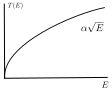
\includegraphics[scale=0.8]{moderna-img/energia.png}
\end{figure}
Fendas em um anteparo de chumbo (Pb) foram colocadas na frente do feixe de raios $X$ espalhados pelo alvo de grafite, a fim de selecionar o ângulo $\theta$. Abaixo são fornecidas as seções de choque do Pb como função da energia para os processos de espalhamento ($\sigma_{S}$), de efeito fotoelétrico ($\sigma_{PE}$) e de produção de pares ($\sigma_{PR}$), bem como o valor total ($\sigma$).
\begin{figure}[H]
\centering
\includegraphics[scale=0.8]{moderna-img/energia2.png}
\end{figure}
c) Na energia escolhida para o experimento, qual processo de absorção do feixe pelo chumbo tem a maior contribuição na atenuação?
d) Para que valores aproximados de energia os efeitos de espalhamento predominam sobre os outros processos de absorção no chumbo?
e) Estime a espessura do anteparo de chumbo para que ele atenue a intensidade do feixe incidente de um fator igual a $e^{-3}$. Para esse cálculo considere que o chumbo possui uma densidade aproximada de $3 \times 10^{22}$ $átomos/cm^{3}$.
f) Um monocristal de silício com distância interplanar de aproximadamente $0,31 \ nm$ é escolhido como espectrômetro do experimento. Determine o menor ângulo que o feixe espalhado pelo alvo de grafite deve fazer com a superfície do monocristal para que o feixe seja difratado em direção ao detector.




\item Utilizando o modelo de Bohr:

a) Deduza a expressão para os níveis de energia do íon $He^{+}$ ($Z = 2$, $M_{He^{+}} >> m_{e}$) e calcule os valores das energias até $n = 5$.

Com os resultados deste item, determine:

b) a energia de ionização do $He^{+}$,
c) o comprimento de onda de uma linha de emissão do $He^{+}$ na região do espectro visível,
d) Dois íons de $He^{+}$ no estado fundamental e com mesma energia cinética colidem frontalmente. Cada qual emite um fóton de comprimento de onda $120 \ nm$ e fica com energia cinética final nula, no estado fundamental. Qual é a velocidade dos íons antes da colisão?




\item Uma fonte produz um feixe de nêutrons com energia cinética média de 0,0133 $eV$ e incerteza relativa na velocidade, $\Delta v/v$, de $1 \times 10^{-4}$. Num determinado instante, a função de onda unidimensional de um nêutron é descrita por um pacote de ondas dado por
$$
\psi(x) = A exp \left(  -\frac{x^{2}}{2 (\Delta x)^{2}}  \right) exp(i k_{0} x)
$$
Nesta expressão, $A$ é uma constante, $\Delta x$ é a incerteza padrão na posição, e $\hbar k_{0}$ é o momento linear médio.

a) Estime o comprimento de onda de de Broglie do nêutron e identifique a região do espectro eletromagnético correspondente a esse comprimento de onda.
b) Estime a temperatura associada a essa fonte de nêutrons.
c) Determine a constante $A$, expressando-a em termos de $\Delta x$.
d) Com um pacote de ondas desse tipo, o produto das incertezas na posição e no momento é o mínimo permitido pelo princípio da incerteza. Estime $\Delta x$ neste caso.



\item Átomos muônicos são formados por um núcleo de carga $Ze$, com o muon negativo orbitando ao redor do núcleo. O muon possui carga igual à do elétron, mas massa 207 vezes maior que a deste. Para um átomo muônico cujo núcleo é formado por apenas um próton ($m_{p} = 1836 m_{e}$), estime:

a) a massa reduzida do sistema, em termos da massa do elétron $m_{e}$.
b) o raio da primeira órbita de Bohr desse átomo muônico,
c) o comprimento de onda da primeira linha da série de Lyman, sabendo que
$$
\frac{1}{\lambda} = R_{\mu} \cdot \left(  1 - \frac{1}{n_{i}^{2}}  \right)
$$
onde $R_{\mu}$ é a constante de Rydberg para o átomo muônico.
d) Qual é a região do espectro eletromagnético que permite estudar a emissão da série de Lyman desse átomo muônico?




\item Suponha que após uma colisão Compton entre um fóton e um elétron inicialmente em repouso, o fóton e o elétron saiam de maneira simétrica, ou seja, com ângulos de valores iguais $\theta$  mas opostos em relação à direção original de incidência do fóton. Se a energia inicial do fóton é de 30 $keV$, qual o ângulo $\theta$ que corresponde a esse espalhamento simétrico e qual o valor das energias finais do fóton e elétron?


\item Quando uma amostra sólida do metal de sódio é iluminada com luz de comprimento de onda $4.2 \times 10^{2} \ nm$, o potencial necessário para que não flua corrente no circuito abaixo é de 0.65 $V$. Quando o comprimento de onda da luz é alterado para $3.1 \times 10^{2} \ nm$, o mesmo potencial agora vale 1.69 $V$. Encontre a função trabalho do sódio e o valor da constante de Planck.
\begin{figure}[H]
\centering
\includegraphics[scale=0.8]{moderna-img/sodio.png}
\end{figure}


\item Dois irmãos gêmeos, Antônio e Bruno, dezem possuir uma ligação cósmica que faz com que um sinta as dores do outro, instantaneamente. Esses dois irmãos estão em repouso em um dado referencial, separados por uma distância de 500 $km$, e Antônio começa a chorar exatamente no instante em que Bruno acerta o dedo com um martelo. Um cientista viajando com a velocidade de $(12/13)c$ ao longo da linha que une os dois irmãos, indo de Antônio para Bruno observa os dois eventos (choro de Antônio, martelada de Bruno). Qual a sequência dos eventos segundo o cientista (forneça a diferença de tempo entre eles, se eles não forem simultâneos)? É possível concluir se a "ligação cósmica" realmente existe entre os irmãos?


\item Positrônio é um átomo formado por um elétron e um pósitron (anti-életron). Ele é semelhante ao átomo de hidrogênio, com o pósitron no lugar do próton. Utilizando o modelo de Bohr, responda:

a) Encontre o raio de Bohr para esse sistema.
b) Qual o comprimento de onda de um fóton associado à transição $n=2$ para $n=1$?




\item Duas partículas de mesma massa de repouso $m_{0}c^{2} = 1 \ GeV$ caminham em sentidos opostos com velocidades de $0,6c$ respectivamente. Num determinado instante elas colidem formando uma única partícula de massa de repouso $M_{0}$ e velocidade $V$. Determine:

  a) o valor de $M_{0}$;
  b) o valor de $V$;
  c) a energia cinética da partícula formada na colisão.




\item (a) O tempo de vida do Sol pode ser estimado a partir da massa disponível para combustão nuclear e da taxa de energia irradiada ou luminosidade, $L = 4 \times 10^{26} \ W$. A massa disponível é a massa do núcleo do Sol (região com temperatura suficientemente alta para haver fusão nuclear), que equivale a $10\%$ da massa total $(M_{total} = 2 \times 10^{30}) \ kg$ do Sol. Supondo que esse núcleo solar é formado por prótons que se fundem dando origem ao $^{4}He$ e que este processo é o mais relevante para o balanço energético, estime o tempo de vida do Sol.


  b) Tendo a luminosidade do Sol acima, estime a temperatura de equilíbrio da Terra.




\item Um possível modelo para um nêutron seria um elétron e um próton mantidos juntos pela atração coulombiana. Supondo um raio para o nêutron de $10^{-15} \ m$, faça uma estimativa da energia cinética do elétron e compare com a energia potencial eletrostática. Comente se esse modelo de nêutron é razoável. (Note que o valor da velocidade do elétron irá exigir estimativas relativísticas para a energia cinética.)


\item Suponha um carro de 1000 $kg$ atravessando uma praça de pedágio a uma velocidade de 36 $km/h$ (sem parar). Supondo que a largura das cabines de pedágio é de 5 $m$, diga qual deveria ser a ordem de grandeza da constante de Planck $h$ para observarmos efeitos de difração na passagem do carro.




\item Quando o comprimento de onda da luz incidente excede 650 $nm$, a emissão de fotoelétrons de uma superfície não é observada. Se a mesma superfície é agora irradiada com luz de comprimento de onda de 390 $nm$, qual a máxima energia dos fotoelétron emitidos?


\item Suponha que uma pedra de 100 $kg$ esteja flutuando no espaço. Considere que um nêutron é atraído gravitacionalmente por essa pedra e, devido à força gravitacional, fica orbitando em torno da pedra em uma órbita circula. Aplique a teoria de Bohr para o sistema e encontre a energia do estado fundamental. Encontre o raio orbital do estado fundamental.


\item Uma barra de metal inicialmente a uma temperatura de 100 $K$ é colocada no espaço interestelar. Qual a temperatura (aproximada) final da barra. Através de qual mecanismo físico essa temperatura é atingida?



\item Durante o processo de fotossíntese, um dos picos no espectro de absorção das moléculas de clorofila tem comprimento de onda $\lambda_{vermelha} = 6,6 \times 10^{-7} \ m$, correspondendo à luz vermelha. Após a absorção desses fótons, há basicamente três possíveis rotas de conversão de energia: 1) reemissão de fótons; 2) conversão em calor; ou 3) o processo fotossintético propriamente dito, com utilização da radiação incidente para armazenar energia química. Considerando uma eficiência de 80 $\%$ no processo de fotossínteses (80 $\%$ dos fótons absorvidos resultam no armazenamento de energia), calcule o número necessário de fótons absorvidos para que ocorra um armazenamento de energia química total de $1,0 \ J$ na planta.


\item Considere que uma pessoa tem uma área de pele de aproximadamente 1,5 $m^{2}$, a uma temperatura de aproximadamente 320 $K$. Considere essa pessoa como um corpo negro ideal.

  a) Calcule a potência (em watts) irradiada por essa pessoa.
  b) Suponha que essa pessoa esteja nua em um ambiente cuja temperatura seja de 300 $K$. Qual a taxa líquida de perda de energia no estado estacionário (em watts)?
  c) Em um dia (24 horas) qual seria, portanto, a quantidade de energia perdida por radiação, na situação do item (b)?
  \item[] Compare seu número com uma alimentação de $2 \times 10^{3} \ kcal$ ($8 \times 10^{3} \ kJ $) por dia.




\item Pedro e João estão no laboratório de Física utilizando um aparado experimental que incide radiação eletromagnética de frequência $\nu = 1,0 \times 10^{15} \ Hz$ em um material cuja função trabalho vale $5,0 \ eV$. Para o desapontamento dos estudantes, nenhuma fotocorrente é detectada. João sugere que a intensidade da radiação seja aumentada.

  a) Isso irá resolver o problema? Justifique.
  b) Se não resolver, qual a sua sugestão para que exista uma fotocorrente não nula?




\item Uma barra, em repouso no sistema inercial $S$, possui comprimento próprio $L$ e está inclinada de um ângulo $\theta$ em relação ao eixo $x$ do referencial $S$. Um outro referencial $S'$ move-se com velocidade $\vec{v} = 0,6 c \hat{i}$ em relação a $S$.

  a) Qual é o comprimento $L'$ da barra medido por um observador em repouso em "S'"?
  b) Qual é o ângulo $\theta '$ formado entre a barra e o eixo $x'$ do referencial $S'$, medido no sistema $S'$?



\item A fonte de energia do Sol depende basicamente da conversão de quatro núcleos de $H$ (prótons) em um núcleo de $^{4}He$ (2 prótons e 2 nêutrons). Em uma das chamadas cadeias próton-prótons ($ppl$), cada fusão total de 4 prótons, que gera um núcleo de $^{4}He$, produz um total de dois neutrinos. Neutrinos basicamente não interagem com a matéria e portanto podem escapar do Sol e, eventualmente, ser detectados na Terra. Considerando que: 1) o valor da taxa de energia irradiada pelo Sol, ou luminosidade, vale $L = 4 \times 10^{26} W$; 2) somente a cadeia $ppI$ contribui para a geração de energia no Sol; e 3) cerca de 0,7 $\%$ da massa de repouso total dos prótons é liberada como energia na cadeia $ppI$, responda:

  a) Quantos neutrinos são produzidos no Sol por segundo?
  b) Quantos chegam à Terra por segundo?



\item Uma átomo de deutério, que se encontra inicialmente em repouso no estado $n=3$, faz transição para o estado fundamental, $n=1$.

  a) Mostre que a velocidade de recuo do átomo devida à emissão do fóton é dada aproximadamente por $v = 8hR/9M$, onde $R$ é a constante de Rydberg e $M$ a massa do átomo.
  b) Estime a porcentagem da energia da transição $3 \rightarrow 1$ que é carregada pelo átomo de deutério em recuo. (Dê o resultado com 1 algarismo significativo.)



\item Uma partícula de massa de repouso $M_{0}$ se move com velocidade $V = V \hat{x} $ tal que sua energia cinética é de $\frac{1}{4} M_{0} c^{2}$ no referencial do laboratório. Num determinado instante, ela se desintegra em duas partículas idênticas de massa $m_{0} = \frac{3}{10}M_{0}$ que se movem paralelamente ao eixo $x$. Determine:

a) A velocidade $V$ da partícula $M_{0}$, antes do decaimento, no sistema do laboratório.
b) As velocidades $u'_{1}$ e $u'_{2}$ das partículas de massa $m_{0}$ no referencial do seu centro de massa ($CM$).
c) As velocidades $u_{1}$ e $u_{2}$ das duas partículas no referencial do laboratório.
d) Repita os cálculos do ítem (c), considerando agora que no referencial do $CM$ as partículas são emitidas com velocidades ao longo do eixo $y'$.



\item Mostre que o comprimento de onda de de Broglie de uma partícula de carga $e$ e massa de repouso $m_{0}$, acelerada a partir do repouso e adquirindo velocidades relativísticas, é dada como função do potencial acelerador $V$ pela expressão
$$
\lambda = \frac{h}{\sqrt{2m_{0} eV}} \left( 1 + \frac{eV}{2m_{0}c^{2}}   \right)^{1/2}.
$$



\item Um feixe fino de $1,0 \times 10^{6}$ partículas $\alpha$ por segundo, com energia de 5,0 $MeV$, incide normalmente num alvo de Cu ($Z = 29$, $A = 60$, densidade 9 $g/cm^{3}$) de $1,0 \times 10^{-4} \ cm$ de espessura. As partículas espalhadas coulombianamente são observadas numa tela fluorescente de $4 \times 4 \ mm^{2}$, colocada a 10 $cm$ do centro do alvo numa direção fazendo um ângulo de $60º$ com a do feixe incidente. (Este foi um dos casos estudados por Geiger e Marsden.) Nos ítens abaixo utilize apenas um ou dois algarismos significativos.

\item[] Dados: Espalhamento de Rutherford $$  dN = \left(  \frac{zZe^{2}}{4 \pi \epsilon_{0}} \frac{1}{4 E}  \right)^{2}  \frac{n I}{\operatorname{sen}^{4}(\theta/2) } d \Omega $$
  a) Determine o valor da densidade de átomos de cobre por unidade de área no alvo.
  b) Qual é a dimensão do parâmetro  $\frac{zZe^{2}}{16 \pi \epsilon_{0} E}$? Calcule o seu valor.
  c) Calcule o número de cintilações por minuto observadas na tela.




\item Um átomo de hidrogênio está em seu primeiro estado excitado ($n = 2$). Usando o modelo de Bohr para o átomo, calcule as grandezas abaixo, expressando seus resultados nas unidades que achar conveniente:

a) o raio da órbita do elétron,
b) o momento linear do elétron,
c) o momento angular do elétron,
d) sua energia cinética,
e) sua energia potencial.



\item A vida-média própria de um píon é $3,6 \times 10^{-8} \ s$. Se um feixe de píons tem velocidade de $0,8c$:

a) qual é a vida-média das partículas no referencial do laboratório?
b) que distância elas percorrem, em média, antes de se desintegrarem?
c) qual seria a resposta do ítem (b) se não existissem efeitos relativísticos?



\item A figura abaixo corresponde à radiância espectral de dois corpos mantidos a temperaturas $T_{1}$ e $T_{2}$. Vamos supor que a emissão de radiação desses corpos é igual a de corpos negros nessas temperaturas.
\begin{figure}
  \centering
  \includegraphics[scale=0.8]{moderna-img/radiancia.png}
\end{figure}

a) Sabendo que a temperatura do corpo 1 é $T_{1} = 2898 \ K$, determine a temperatura do corpo 2.
b) Qual é a razão entre as potências totais irradiadas pelos corpos, ou seja, quanto vale $R_{2}/R_{1}$, onde $R$ é a radiância total?
c) Segundo a teoria clássica da emissão de radiação do corpo negro, que aspectos das curvas ao lado não podem ser explicados? Como Planck resolveu esse problema?





\item Uma espaçonave de comprimento próprio $L = 300 \ m$ está passando por uma estação transmissora fixa na Terra, a uma velocidade $v = 0,6c$. No instante em que o nariz da espaçonave passa pelo transmissor, dois relógios, um no transmissor e outro no nariz da espaçonave são sincronizados para $t = t' = 0$. No momento em que a cauda da espaçonave passa pelo transmissor, um sinal é enviado pelo transmissor e subsequentemente detectado por um receptor no nariz da espaçonave.

a) Em que instante o sinal foi enviado, segundo o relógio no nariz da espaçonave?
b) Em que instante o sinal foi recebido, segundo o relógio de bordo?
c) Em que instante o sinal foi recebido na espaçonave, segundo o relógio do transmissor?
d) Onde estava o nariz da espaçonave, no instante em que o sinal foi recebido, do ponto de vista de um observador fixo na posição do transmissor.





\item Um átomo de hidrogênio que se encontra no estado fundamental (isto é, de menor energia) é excitado até o estado com $n = 4$.

a) Calcule a energia absorvida pelo átomo.
b) Calcule as energias dos diferentes fótons que podem ser emitidos quando o átomo voltar para o estado fundamental. Faça um diagrama de níveis de energia, indicando essas transições.
c) Calcule a velocidade de recuo do átomo de hidrogênio, ao fazer a transição do estado $n = 4$ diretamente para o estado fundamental. Suponha o átomo em repouso, antes da transição ocorrer.


\item A função de distribuição de velocidades de um grupo de $N$ partículas é dada por $dN_{v} = av dv$ onde $dN_{v}$ é o número de partículas que tem velocidades entre $v$ e $v + dv$, e $a$ é uma constante. Nenhuma partícula tem velocidade maior que $V$ , sendo que as velocidades podem variar entre $0$ e esse valor máximo, $V$.

a) Esboce o gráfico da função de distribuição, ou seja $g(v) = d N_{v}/dv$ em função de $v$.
b) Calcule o valor da constante a em termos de $N$ e $V$.
c) Calcule a velocidade média, a velocidade quadrática média e a velocidade mais provável em termos de $V$.
d) Qual porcentagem das partículas tem velocidades entre a velocidade média e $V$? E entre a velocidade quadrática média e $V$?




\item Uma sonda interestelar afasta-se da Terra com velocidade $v = c/3$ e a cada um ano-luz (medido no referencial da sonda) ela emite um sinal luminoso de comprimento de onda $\lambda_{0}$ em direção à Terra. Deseja-se saber,

a) com que periodicidade os sinais chegam à Terra?
b) quanto tempo após o lançamento o primeiro sinal luminoso chega à Terra?
c) onde estará a sonda quando esse sinal chegar à Terra?
d) com que comprimento de onda os sinais são recebidos na Terra?




\item Quando Bohr desenvolveu sua teoria atômica procurou-se dar respaldo a mesma achando-se situações em que ela concordava com resultados experimentais. Consideraremos três dessas aqui, para um átomo monoeletrônico com massa nuclear $M$ finita e número atômico $Z$. Para isso,

a) deduza a expressão (em função das constantes $e$, $m$, $h$, etc) da energia $E_{n}$ dos níveis quantizados, que sabemos reproduz as linhas principais do espectro de átomos monoeletrônicos;
b) calcule a razão $E_{n}(He^{+})/E_{n}(H)$, entre as energias dos níveis eletrônicos do hélio uma vez ionizado ($He^{+}$, $Z=2$, $M=4$ u.a.) para aquelas do hidrogênio ($H$, $Z=1$, $M=1$ u.a.) e
c) mostre que para um número quântico $n$ muito grande, a frequência da luz emitida na transição $n \rightarrow n - 1$  coincide com a frequência clássica de revolução do elétron no $n-$ésimo estado. Isso mostra que a teoria obedece o princípio de correspondência.





\item (a) As seguintes afirmações referem-se ao efeito fotoelétrico. Responda Verdadeiro (V) ou Falso (F) e justifique brevemente a sua resposta (máximo de três linhas). Respostas sem justificativas ou com justificativas erradas não serão consideradas. Responda na folha de Respostas.

\item[1.] Incide-se luz num material fotoelétrico e não se observa a emissão de elétrons. Para que ocorra a emissão de elétrons no mesmo material basta que se aumente suficientemente a intensidade da luz incidente.

\resposta (F) O efeito fotoelétrico associa-se à emissão de elétrons devido à incidência de fótons. A energia cinética máxima desses elétrons é $K_{max} = hf - W$, sendo $W$ a função trabalho do material que emite os elétrons. Não há relação imediata entre intensidade incidente e emissão de elétrons.

\item[2.] Incide-se luz num material fotoelétrico e não se observa a emissão de elétrons. Para que ocorra a emissão de elétrons no mesmo material basta que se aumente suficientemente a frequência da luz incidente.

\resposta (V) O efeito fotoelétrico associa-se diretamente coma frequência do fóton incidente e só ocorre emissão eletrônica a partir de uma frequência dada por $f_{0} = W/h$. Assim que essa frequência for ultrapassada, ocorre emissão eletrônica de forma significativa.

\item[3.] No contexto do efeito fotoelétrico, o potencial de corte é a tensão necessária para deter os elétrons que escapam do metal com a menor velocidade possível.

\resposta (F) O potencial de corte é a tensão necessária para deter os elétrons que escapam do metal com maior velocidade (ou energia cinética) possível

\item[4.] Quando luz azul incide sobre uma placa de zinco, ela não produz efeito fotoelétrico, mas quando iluminada com luz vermelha ocorre emissão de elétrons.

\resposta (F) Quando a frequência diminui, se antes não se produzia efeito fotoelétrico, este não deve passar a ocorrer.

\item[5.] Quanto maior for a frequência da luz incidente, maior será a energia cinética dos elétrons emitidos.

\resposta (V) Sim, estatisticamente falando, de acordo com a relação $K_{max} = hf - W$

b) Considere o efeito fotoelétrico inverso, ou seja, a emissão de fótons em consequência do bombardeio de um material com elétrons de alta velocidade. Calcule a frequência máxima que podem ter os fótons emitidos se a superfície é bombardeada com elétrons com velocidade $c/2$, onde $c$ é a velocidade da luz.





\item A energia da radiação de corpo negro, por unidade de volume e por unidade de intervalo de frequência, é dada por:
$$ u_{\nu} = \frac{8 \pi h}{c^{3}} \frac{\nu^{3}}{e^{\frac{\hbar \nu}{k_{B} T}} - 1} $$
onde $\nu$ representa a frequência do fóton e $T$ a temperatura da radiação.

a) Deduza a expressão para a energia total $E$ de um gás de fótons em um volume $V$. Qual é a dependência de $E$ com a temperatura?

\resposta Conforme informa o enunciado:
$$
\frac{E}{V} = \int_{0}^{\infty} u_{\nu} (\nu) d \nu = \int_{0}^{\infty} \frac{8\pi h}{c^{3}} \frac{\nu^{3}}{e^{h \nu / k_{B} T} - 1} d\nu
$$
Utilizando a mudança de variável:
$$
\nu = \frac{k_{B} T w}{h} \Rightarrow d \nu = \frac{w^{3}}{e^{w}-1} dw
$$
Da igualdade acima já é possível concluir que $E \propto T^{4} $. Mas vamos continuar o problema... Como sabemos:
$$
\int_{0}^{\infty} \frac{w^{3}}{e^{w}-1} dw = \frac{\pi^{4}}{15}
$$
De forma que:
$$
\frac{E}{V} = \frac{8 \pi (k_{B} T)^{4}}{(ch)^{3}} \frac{\pi^{4}}{15}
$$

\begin{figure}
  \centering
  \includegraphics[scale=0.8]{moderna-img/funcao}
  \caption{Gráfico da função $f(w) = \frac{w^{3}}{e^{w}-1}$, com $\gamma \approx 2,82144$ sendo o ponto de máximo. A área sob esta curva quando integrada de 0.}
\end{figure}
Se soubermos que:
$$
\frac{8 \pi^{5}k_{B}^{4} }{15(ch)^{3}} = \frac{4 \sigma}{c}
$$
Sendo $\sigma$ a constante de Stefan-Boltzmann, temos:
$$
\frac{E}{V} = \frac{4 \sigma T^{4}}{c} \ \Rightarrow \ E = \frac{4 V \sigma T^{4}}{c} \propto T^{4}
$$
OBS.: obviamente, nessa questão, não é necessário saber o valor da integral, basta saber que ela converge e fornece um número como resultado, já que este item só pede qual é a dependência de $E$ com $T$. Pela mesma razão não é necessário saber quanto vale a constante de Boltzmann.


b) Esboce gráficos de $u_{\nu}(\nu)$ para duas temperaturas $T_{1}$ e $T_{2}$, sendo $T_{1} < T_{2}$.

\resposta Quando $\nu \rightarrow \infty$, $\lim_{\nu \rightarrow \infty} u_{\nu} (\nu) \rightarrow 0$.
Quando $\nu \rightarrow 0$, $\lim_{\nu \rightarrow 0} u_{\nu} (\nu) \rightarrow 0$.

(Observe que é mais fácil notar que as afirmações acima estão corretas se usarmos as aproximações:$ \lim_{\nu \rightarrow \infty} u_{\nu} (\nu) \sim
\lim_{\nu \rightarrow \infty} A \nu^{3} e^{-h\nu/k_{B}T}$; $ \lim_{\nu \rightarrow 0} u_{\nu} (\nu) \sim
\lim_{\nu \rightarrow 0} B \nu^{2} \rightarrow 0$, com $A$ e $B$ constantes adequadas.)

Para $\alpha > 0$ e $T_{2} > T_{1} > 0$, podemos concluir que:
$$
T_{2} > T_{1} \Rightarrow \frac{1}{T_{2}} < \frac{1}{T_{1}} \Rightarrow  \frac{\alpha}{T_{2}} < \frac{\alpha}{T_{1}} \Rightarrow e^{\alpha/T_{2}} > e^{\alpha/T_{1}} - 1 > e^{\alpha/T_{2}} - 1
$$
$$
\Rightarrow \frac{1}{e^{\alpha/T_{1}} -1} < \frac{1}{e^{\alpha/T_{2}} -1} \Rightarrow u_{\nu}(\nu, T_{2}) > u_{\nu}(\nu, T_{1}), \forall \ \nu \in \mathbb{R}^{+}
$$
O máximo de $u_{\nu}(\nu)$ segue a lei de Wien:
$$
\lambda_{max} = \frac{c}{\nu_{max}} = \frac{b}{T} \Rightarrow \nu_{max} = \frac{cT}{b}
$$
Com $b$ é a constante do deslocamento de Wien e $c$ é a velocidade da luz. Para perceber a diferença na emissão espectral, veja o gráfico.
\begin{figure}[H]
  \centering
  \includegraphics[scale=0.8]{moderna-img/densidade.png}
  \caption{Gráfico da densidade de energia por frequência versus a frequência. Note que $k$ é a constante de Boltzmann $\zeta = \frac{8 \pi k^{3}}{c^{3} h^{2}}$, $\xi = \frac{k}{h}$, $\gamma \approx 2,82144$.}
\end{figure}



c) Escreva as formas assintóticas de $u_{\nu}(\nu)$ no caso de frequências muito altas (lei de radiação de Wien) e no caso de frequências muito baixas (lei de radiação de Rayleigh-Jeans).

\resposta Para frequências muito altas, a forma assintótica para $\nu \Rightarrow \infty$ é dada por:
$$
u_{\nu} (\nu >> \nu_{\max}) \approx \frac{8\pi h}{c^{3}} \nu^{3} e^{-h \nu/k_{B} T}
$$
Essa é a lei de radiação de Wien. Para frequências muito baixas, a forma assintótica para $\nu \rightarrow 0$ é dada por:
$$
u_{\nu} (\nu << \nu_{\max}) \approx \frac{8\pi k_{B} T}{c^{3}} \nu^{3}
$$
Essa é a lei de radiação de Rayleigh-Jeans.



d) Imagine que o Universo seja uma cavidade esférica de paredes impenetráveis e raio $10^{28} cm$, contendo um gás de fótons em equilíbrio térmico. Se a temperatura dentro da cavidade for de $3 K$, estime a quantidade de energia contida nessa cavidade.

\resposta Como $E = \frac{4 \sigma}{c} T^{4} V$. Para uma esfera: $V = \frac{4 \pi}{3} r^{3}$. Assim, como: $\sigma \approx 5,67 \times 10^{-8} \ W/m^{2} K^{4}$, $c \approx 3 \times 10^{8} \ m/s$, $T = 3K$ e $V \approx 4,19 \times 10^{78} \ m^{3}$. Temos:

$$E \approx 2,57 \times 10^{65} \ J $$

\begin{figure}[H]
  \centering
  \includegraphics[scale=0.7]{moderna-img/jeans.png}
  \caption{Gráfico da densidade de energia por freqüência versus a freqüência para as diversas leis de radiação (com $T$ constante, e $k_{B}$ a constante de Boltzmann, e $e$ é o numero Neperiano). Lembrando que $\gamma \approx 2,82144$. Note como as leis de radiação de Rayleigh-Jeans e de Wien concordam com a lei de Planck, nos limites assintóticos apropriados.}
\end{figure}


e) Supondo que o Universo se expanda adiabaticamente, calcule a temperatura que ele terá quando o seu volume for o dobro do valor atual (a entropia do gás de fótons é $S \propto V T^{3}$).

\resposta Numa expansão adiabática:
$$
\delta Q = T dS = 0 \Rightarrow dS = 0
$$
Mas, se $C$ e $G$ são constantes adequadas:
$$
S = CVT^{3} \Rightarrow dS = CT^{3} dV + 3 C T^{2} V dT = 0 \Rightarrow CT^{3} dV = -3CT^{2}V dT \Rightarrow
$$
%
$$
\frac{dV}{V} = -3 \frac{dT}{T} \Rightarrow \mathrm{ln} V = -3 \mathrm{ln} T + \mathrm{ln} G \Rightarrow V = GT^{-3}
$$
Assim: $T_{0} = \left( \frac{G}{V_{0}} \right)^{1/3}$. De forma que: $T_{f} = \left( \frac{G}{2V_{0}} \right)^{1/3} = \left( \frac{1}{2} \right)^{1/3} T_{0} \approx 2,38 K$.








\item Um elétron de massa de repouso $m$, e carga elétrica $-e$, está em repouso na origem de um referencial $S$. Num dado momento liga-se um camp o elétrico constante e uniforme de intensidade $E$. De acordo com a teoria especial da relatividade de Einstein:

a) Qual a velocidade do elétron em função do tempo, no referencial $S$?
b) Qual o valor desta velocidade para tempos muito grandes?
c) Qual será a distância do elétron à origem em função do tempo, medido no referencial $S$ a partir do momento em que o camp o é ligado?
d) Se o camp o elétrico permanecer ligado por um temp o $T$, qual será a energia total do elétron, no referencial $S$, após o camp o elétrico ser desligado?
e) Qual a velo cidade do elétron, após o campo ser desligado, medida em um referencial $S'$ que se move com velocidade $v_{0}$ na direção e sentido do campo elétrico?




\item Considere um corp o negro esférico de raio $r$ colocado em órbita circular em torno do Sol, e com o raio da órbita sendo igual à distância Terra-Sol. Considere que a temperatura na superfície do Sol é de 5700°$C$. Responda:

a) Qual a potência total emitida pelo Sol?
b) Qual a potência total emitida pelo corpo negro em equilíbrio com a radiação solar para $r = 1\ m$?
c) Qual é a temperatura em que o corpo negro entra em equilíbrio com a radiação solar?
d) Qual é a frequência da radiação emitida com maior intensidade pelo corpo negro?

Observação: supomos que a temperatura do corpo negro, ao entrar em equilíbrio com a radiação solar, é a mesma em todos os seus pontos. Ou seja, supomos que o seu raio $r$ não é muito grande, e sua condutividade térmica não é muito pequena.




\end{enumerate}


























